\documentclass[12pt]{article}

% Extract
\usepackage[active,
            generate=topology_definitions,
            %extract-cmd={section},
            extract-env={definition,algorithm}]{extract}

% \usepackage[active,
%             generate=topology_theorems,
%             %extract-cmd={section},
%             extract-env={theorem,corollary,claim}]{extract}

\begin{extract*}

%%%%%%%%%%%%%%%%%%%%%%%%%%%%%%%%%%%%%%%%%%%%%%%%%%%%%%%%%%%%%%%%%%%%%%%%%%%%%%%%%%

% Packages

% AMS 
\usepackage{amsmath, amssymb, amsthm, amsbsy}
% Geometry
\usepackage{geometry}
% Colors
\usepackage[usenames,dvipsnames]{xcolor}
% Figures
\usepackage{graphicx}
\usepackage{float}
% Multi column lists
\usepackage{multicol}
% Subfigures
\usepackage{caption}
\usepackage{subcaption}
% Caligraphic
\usepackage{mathrsfs}
\usepackage{bbm}
% Bold
\usepackage{bm}
% algos
\usepackage[linesnumbered, lined, ruled]{algorithm2e}
% Spacing 
\usepackage{setspace}
% Refs/links
\usepackage[colorlinks=true, citecolor=Blue, linkcolor=blue]{hyperref}
\newcommand\myshade{85}
\colorlet{mylinkcolor}{violet}
\colorlet{mycitecolor}{PineGreen}
\colorlet{myurlcolor}{Aquamarine}

\hypersetup{
  linkcolor  = mylinkcolor!\myshade!black,
  citecolor  = mycitecolor!\myshade!black,
  urlcolor   = myurlcolor!\myshade!black,
  colorlinks = true,
}
% Bibliography
\usepackage{filecontents}
\usepackage{natbib}
% Indent
\usepackage{indentfirst}
% Pretty lists
\usepackage{enumitem}
\setlist[enumerate]{itemsep=2pt,topsep=3pt}
\setlist[itemize]{itemsep=2pt,topsep=3pt}
\setlist[enumerate,1]{label=(\roman*)}

% Code
\usepackage{listings}

% Appendix
\usepackage[toc,page]{appendix}

% Math
\usepackage{mathtools}
\usepackage{xparse}


%%%%%%%%%%%%%%%%%%%%%%%%%%%%%%%%%%%%%%%%%%%%%%%%%%%%%%%%%%%%%%%%%%%%%%%%%%%%%%%%%%

% Document Settings

% Figure path
\graphicspath{{./figures/}}
% Matrix columns
\setcounter{MaxMatrixCols}{10}
% So pages will break inside long equation environments
\allowdisplaybreaks
% Font
\usepackage{mathpazo} 
\linespread{1.05}  
%\usepackage{courier}
% Geometry
\geometry{left=1in,right=1in,top=1in,bottom=1in}
% Counters
\setcounter{tocdepth}{2}
\setcounter{secnumdepth}{3}

%%%%%%%%%%%%%%%%%%%%%%%%%%%%%%%%%%%%%%%%%%%%%%%%%%%%%%%%%%%%%%%%%%%%%%%%%%%%%%%%%%

% Colors

\definecolor{Tm}{rgb}{0,0,0.80}
\newcommand{\navy}[1]{\textcolor{MidnightBlue}{\bf #1}}

%%%%%%%%%%%%%%%%%%%%%%%%%%%%%%%%%%%%%%%%%%%%%%%%%%%%%%%%%%%%%%%%%%%%%%%%%%%%%%%%%%

% Environments

\theoremstyle{plain}
\newtheorem{theorem}{\color{ForestGreen}{\textbf{Theorem}}}[section]
\newtheorem{lemma}[theorem]{\color{ForestGreen}{\textbf{Lemma}}}
\newtheorem{proposition}[theorem]{\color{ForestGreen}{\textbf{Proposition}}}
\newtheorem{corollary}[theorem]{\color{ForestGreen}{\textbf{Corollary}}}
\newtheorem{axiom}[theorem]{\color{ForestGreen}{\textbf{Axiom}}}
\newtheorem{conjecture}[theorem]{Conjecture}
\newtheorem{case}[theorem]{Case}
\newtheorem{conclusion}[theorem]{Conclusion}
\newtheorem{criterion}[theorem]{Criterion}
\newtheorem{notation}[theorem]{Notation}
\newtheorem{problem}[theorem]{Problem}

\theoremstyle{definition}
\newtheorem{definition}{\color{MidnightBlue}{\textbf{Definition}}}[section]
\newtheorem{example}{\color{WildStrawberry}Example}[section]
\newtheorem{assumption}{Assumption}[section]
\newtheorem{condition}[assumption]{Condition}
\newtheorem*{solution}{\color{Goldenrod}Solution}
% \newenvironment{solution}[1][\proofname]{%
%   \proof[\bf \color{Goldenrod}Solution to #1]%
% }{\endproof}

\newtheorem{exercise}{\color{YellowOrange}Exercise}[section]

% Literature Summary Standards
\newtheorem*{motivation}{Motivation}
\newtheorem*{summary}{Summary}
\newtheorem*{remark}{Remark}
\newtheorem*{model}{Model}
\newtheorem*{tresults}{Theoretical Results}
\newtheorem*{eresults}{Empirical Results}

%%%%%%%%%%%%%%%%%%%%%%%%%%%%%%%%%%%%%%%%%%%%%%%%%%%%%%%%%%%%%%%%%%%%%%%%%%%%%%%%%%

% Math macros

% Math ``brackets''
\newcommand\parens[1]{\left( #1 \right)}
\newcommand\squares[1]{\left[ #1 \right]}
\newcommand\braces[1]{\left\{ #1 \right\}}
\newcommand\angles[1]{\left\langle #1 \right\rangle}
\newcommand\ceil[1]{\left\lceil #1 \right\rceil}
\newcommand\floor[1]{\left\lfloor #1 \right\rfloor}
\newcommand\abs[1]{\left| #1 \right|}
\newcommand\dabs[1]{\left\| #1 \right\|}
\newcommand\vect[1]{\mathbf{#1}}
\newcommand\closure[1]{\overline{#1}}
\newcommand\pset[1]{\mathcal{P}\left(#1\right)}
\newcommand\inv[1]{#1^{-1}}
\newcommand\norm[1]{\lVert#1\rVert}

% inner product
\providecommand{\inner}[1]{\left\langle{#1}\right\rangle}
% stochastic dominance
\newcommand{\lesd}{\preceq_{\textrm{SD}}}

% Set builder (use \Set ultimately and separate by ;)
\DeclarePairedDelimiterX{\set}[1]{\{}{\}}{\setargs{#1}}
\NewDocumentCommand{\setargs}{>{\SplitArgument{1}{;}}m}
{\setargsaux#1}
\NewDocumentCommand{\setargsaux}{mm}
{\IfNoValueTF{#2}{#1} {#1\nonscript\:\delimsize\vert\allowbreak\nonscript\:\mathopen{}#2}}%
\def\Set{\set*}%

% Shortcut math
\newcommand{\ls}{\leqslant}
\newcommand{\gs}{\geqslant}
\def\ss{\subset}
\def\nss{\not \ss}
\def\sps{\supset}
\def\pss{\subsetneq}
\def\prece{\preccurlyeq}
\def\condgap{\hspace{1cm}}
\def\eprec{\preceq}
% argmax and min
\newcommand{\argmax}{\operatornamewithlimits{argmax}}
\newcommand{\argmin}{\operatornamewithlimits{argmin}}
\newcommand{\es}{\emptyset}
% Implication and reverse implication
\def\imp{\Rightarrow}
\def\pmi{\Leftarrow}
% Integers up to number
\newcommand\intsfin[1]{\braces{1, \ldots, #1}}
% Logic
\def\bic{\Leftrightarrow}
% Bold and italic
\newcommand\boldit[1]{\textbf{\textit{#1}}}
% Misc math
\newcommand{\st}{\ensuremath{\ \mathrm{s.t.}\ }}
\newcommand{\setntn}[2]{ \{ #1 : #2 \} }
\newcommand{\cf}[1]{ \lstinline|#1| }
\newcommand{\fore}{\therefore \quad}
\newcommand{\tod}{\stackrel { d } {\to} }
\newcommand{\tow}{\stackrel { w } {\to} }
\newcommand{\toprob}{\stackrel { p } {\to} }
\newcommand{\toms}{\stackrel { ms } {\to} }
\newcommand{\eqdist}{\stackrel{d} {=} }
\newcommand{\iidsim}{\stackrel{\textrm{ {\sc iid }}} {\sim} }
\newcommand{\1}{\mathbbm 1}
\newcommand{\dee}{\,{\rm d}}
\newcommand{\given}{\, | \,}
\newcommand{\la}{\langle}
\newcommand{\ra}{\rangle}

% Shortcut greek
\def\a{\alpha}
\def\b{\beta}
\def\g{\gamma}
\def\D{\Delta}
\def\d{\delta}
\def\z{\zeta}
\def\k{\kappa}
\def\l{\lambda}
\def\n{\nu}
\def\r{\rho}
\def\s{\sigma}
\def\t{\tau}
\def\x{\xi}
\def\w{\omega}
\def\W{\Omega}
% Nice greek
\newcommand{\p}{\varphi}
\newcommand{\e}{\varepsilon}

% Shorcut vectors
\def\vx{\vect{x}}
\def\vy{\vect{y}}
\def\va{\vect{a}}
\def\vb{\vect{b}}

\newcommand{\CC}{\mathbbm C}
\newcommand{\FF}{\mathbbm F}
\newcommand{\RR}{\mathbbm R}
\newcommand{\NN}{\mathbbm N}
\newcommand{\PP}{\mathbbm P}
\newcommand{\EE}{\mathbbm E}
\newcommand{\TT}{\mathbbm T}
\newcommand{\VV}{\mathbbm V}
\newcommand{\QQ}{\mathbbm Q}
\newcommand{\WW}{\mathbbm W}
\newcommand{\ZZ}{\mathbbm Z}
\renewcommand{\SS}{\mathbbm S}

% Expectation/Probability
\newcommand{\ee}[1]{\mathbbm{E}[{#1}]}
\newcommand{\pp}[1]{\mathbbm{P}({#1})}

\newcommand{\GG}{\mathsf G}
\newcommand{\XX}{\mathsf X}
\renewcommand{\AA}{\mathsf A}
\newcommand{\YY}{\mathsf Y}
\newcommand{\ZZZ}{\mathsf Z}

\newcommand{\aA}{\mathscr A}
\newcommand{\cC}{\mathscr C}
\newcommand{\iI}{\mathscr I}
\newcommand{\eE}{\mathscr E}
\newcommand{\fF}{\mathscr F}
\newcommand{\rR}{\mathscr R}
\newcommand{\sS}{\mathscr S}
\newcommand{\lL}{\mathscr L}
\newcommand{\cG}{\mathscr G}

\newcommand{\pP}{\mathcal P}
\newcommand{\vV}{\mathcal V}
\newcommand{\dD}{\mathcal D}
\newcommand{\mM}{\mathcal M}
\newcommand{\oO}{\mathcal O}
\newcommand{\gG}{\mathcal G}
\newcommand{\hH}{\mathcal H}
\newcommand{\tT}{\mathcal T}
\newcommand{\bB}{\mathcal B}

% Common collections
\def\cA{\col{A}}
\def\cB{\col{B}}
\def\cC{\col{C}}
\def\cT{\col{T}}
\def\cU{\col{U}}

% Common closures
\def\clA{\closure{A}}
\def\clB{\closure{B}}
\def\clK{\closure{K}}

% operators
\DeclareMathOperator{\cl}{cl}
\DeclareMathOperator{\graph}{graph}
\DeclareMathOperator{\interior}{int}
\DeclareMathOperator{\Prob}{Prob}
\DeclareMathOperator{\determinant}{det}
\DeclareMathOperator{\trace}{trace}
\DeclareMathOperator{\sgn}{sgn}
\DeclareMathOperator{\Span}{span}
\DeclareMathOperator{\diag}{diag}
\DeclareMathOperator{\proj}{proj}
\DeclareMathOperator{\rank}{rank}
\DeclareMathOperator{\cov}{Cov}
\DeclareMathOperator{\corr}{Corr}
\DeclareMathOperator{\var}{Var}
\DeclareMathOperator{\mse}{mse}
\DeclareMathOperator{\se}{se}
\DeclareMathOperator{\row}{row}
\DeclareMathOperator{\col}{col}
\DeclareMathOperator{\range}{rng}
\DeclareMathOperator{\kernel}{ker}
\DeclareMathOperator{\dimension}{dim}
\DeclareMathOperator{\bias}{bias}
\DeclareMathOperator{\dom}{dom}
\DeclareMathOperator{\ran}{ran}
\DeclareMathOperator{\Int}{Int}
\DeclareMathOperator{\Cl}{Cl}

\end{extract*}


\title{Topology Notes}
\author{Rebekah Dix}
\begin{document}
\maketitle
\tableofcontents
\newpage 

\section{Set Theory Review}

\begin{definition}[Difference]
	The \navy{difference} of two sets, denoted $A-B$, is the set consisting of those elements of $A$ that are not in $B$. In notation
	\begin{equation*}
		A - B = \{x | x \in A \text{ and } x \not\in B\}	
	\end{equation*}
\end{definition}

\begin{theorem}[Set-Theoretic Rules]
	We have that, for any sets $A, B, C$,
	\begin{enumerate}
		\item First distributive law for the operations $\cap$ and $\cup$:
		\begin{equation}
			A \cap (B \cup C) = (A \cap B) \cup (A \cap C)
		\end{equation}
		\item Second distributive law for the operations $\cap$ and $\cup$:
		\begin{equation}
			A \cup (B \cap C) = (A \cup B) \cap (A \cup C)
		\end{equation}
		\item DeMorgan's laws:
		\begin{equation}
			A - (B \cup C) = (A - B) \cap (A - C)
		\end{equation}
		``The complement of the union equals the intersection of the complements.''
		\begin{equation}
			A - (B \cap C) = (A - B) \cup (A - C)
		\end{equation}
		``The complement of the intersection equals the union of the complements.''
	\end{enumerate}
\end{theorem}


\section{Topological Spaces}

\begin{definition}[Topology, Topological Space]
	A \navy{topology} on a set $X$ is a collection $\tT$ of subsets of $X$ having the following properties:
	\begin{enumerate}
		\item $\emptyset$ and $X$ are in $\tT$.
		\item The union of the elements of any subcollection of $\tT$ is in $\tT$.
		\item The intersection of the elements of any finite subcollection of $\tT$ is in $\tT$.
	\end{enumerate}
	A set $X$ for which a topology $\tT$ has been specified is called a \navy{topological space}.
\end{definition}

\begin{definition}[Open set]
	If $X$ is a topological space with topology $\tT$, we say that a subset $U$ of $X$ is an \navy{open set} of $X$ if $U$ belongs to the collection $\tT$.
\end{definition}

\begin{definition}[Discrete Topology, Trivial Topology]
	If $X$ is any set, the collection of all subsets of $X$ is a topology on $X$, called the \navy{discrete topology}. The collection consisting of $X$ and $\emptyset$ is called the \navy{trivial topology}.
\end{definition}

\begin{example}[Finite Complement Topology]
	Let $X$ be a set. Let $\tT_f$ be the collection of all subsets of $U$ of $X$ such that $X-U$ is either finite or all of $X$. This is topology. We check the three conditions.
	\begin{enumerate}
		\item $X \in \tT_f$ since $X - X$ is the empty set, and hence finite. $\emptyset \in \tT_f$ since $X - \emptyset = X$ is all of $X$.
		\item Let $\{U_\alpha\}$ be an arbitrary of elements of $\tT_f$. Then
		\begin{align*}
			X - \bigcup U_\alpha &= X - \left(U_{\alpha_1} \cup \cdots \cup U_{\alpha_n}  \cdots \right) \\
			&= (X - U_{\alpha_1}) \cap \cdots \cap (X - U_{\alpha_n}) \cdots \\
			&= \bigcap (X - U_\alpha)
		\end{align*}
		Since each $U_\alpha \in \tT_f$, we know that each $X - U_\alpha$ is finite. The intersection of finite sets is finite, so $\{U_\alpha\} \in \tT_f$. 
		\item Let $\{U_i\}$ be a finite collection of sets in $\tT_f$. Then
		\begin{align*}
			X - \bigcap U_i &= X - \left(U_1 \cap \cdots \cap U_n \right) \\
			&= (X - U_1) \cup \cdots \cup (X - U_n) \\
			&= \bigcup (X - U_i)
		\end{align*}
		This is a finite union of finite sets, which is also finite. 
	\end{enumerate}
\end{example}

\begin{definition}[(Strictly) Finer, (Strictly) Coarser, Comparable]
	Suppose $\tT$ and $\tT'$ are two topologies on a given set $X$. If $\tT' \supset \tT$, we say that $\tT'$ is \navy{finer} than $\tT$. If $\tT'$ properly contains $\tT$, we say that $\tT'$ is \navy{strictly finer} than $\tT$. For these respective situations, we say that $\tT$ is \navy{coarser} or \navy{strictly coarser} than $\tT'$. We say that $\tT$ is \navy{comparable} with $\tT'$ if either $\tT' \supset \tT$ or $\tT \supset \tT'$.
\end{definition}


\section{Basis for a Topology}

\begin{definition}[Basis, Basis Elements, Topology $\tT$ generated by $\bB$]
	If $X$ is a set, a \navy{basis} for a topology on $X$ is a collection $\bB$ of subsets of $X$ (called \navy{basis elements}) such that
	\begin{enumerate}
		\item For each $x \in X$, there is at least one basis element $B$ containing $x$.
		\item If $x$ belongs to the intersection of two basis elements $B_1$ and $B_2$, then there is a basis element $B_3$ containing $x$ such that $B_3 \subset B_1 \cap B_2$.
	\end{enumerate}
	If $\bB$ satisfies these two conditions, then we define the \navy{topology $\tT$ generated by $\bB$} as follows: A subset $U$ of $X$ is said to be open in $X$ (that is, to be an element of $\tT$) if for each $x \in U$, there is a basis element $B \in \bB$ such that $x \in B$ and $B \subset U$. Note that each basis element is itself an element of $\tT$.
\end{definition}

\begin{theorem}[Collection $\tT$ generated by a basis $\bB$ is a topology on $X$]
\end{theorem}
\begin{proof}
	We check the three conditions:
	\begin{enumerate}
		\item The empty set is vacuously open (since it has no elements), so $\emptyset \in \tT$. Further, $X \in \tT$ since for each $x \in X$, there must be at least one basis element $B$ containing $x$, which itself is contained in $X$. 
	\end{enumerate}
	\textcolor{red}{[[Incomplete]]}
\end{proof}

\begin{definition}[Subbasis]
	A \navy{subbasis} $\sS$ for a topology on $X$ is a collection of subsets of $X$ whose union equals $X$. The topology generated by the subbasis $\sS$ is defined to be the collection $\tT$ of all unions of finite intersections of elements of $\sS$.
\end{definition}

\section{The Order Topology}

\begin{definition}[Order Topology]
	Let $X$ be a set with a simple order relation, and assume $X$ has more than one element. Let $\bB$ be the collection of all sets of the following types:
	\begin{enumerate}
		\item All open intervals $(a,b)$ in $X$.
		\item All intervals of the form $[a_0, b)$, where $a_0$ is the smallest element (if any) of $X$.
		\item All intervals of the form $(a,b_0]$, where $b_0$ is the largest element (if any) of $X$. 
	\end{enumerate}
	The collection $\bB$ is a basis for a topology on $X$, which is called the \navy{order topology}.
\end{definition}

\begin{proof}[Proof that $\bB$ satisfies the requirements for a basis.] 
	We check the two conditions required to be a basis:
	\begin{enumerate}
		\item Each element contained in a basis element: 
		\item 
	\end{enumerate}
\end{proof}



\section[The Product Topology]{The Product Topology on $X \times Y$}

\begin{definition}[Product Topology]
	Let $X$ and $Y$ be topological spaces. The \navy{product topology} on $X \times Y$ is the topology having as basis the collection $\bB$ of all sets of the form $U \times V$, where $U$ is an open subset of $X$ and $V$ is an open subset of $Y$.
\end{definition}


\section{The Subspace Topology}

\section{Closed Sets and Limit Points}

\begin{definition}[Closed]
	A subset $A$ of a topological space $X$ is said to be \navy{closed} if the set $X - A$ is open.
\end{definition}

\begin{definition}[Interior]
	Given a subset $A$ of a topological space $X$, the \navy{interior} of $A$ is defined as the union of all open sets contained in $A$. Denoted by $\Int A$.
\end{definition}

\begin{definition}[Closure]
	Given a subset $A$ of a topological space $X$, the \navy{closure} of $A$ is defined as the intersection of all closed sets containing $A$. Denoted by $\Cl A$ or $\bar{A}$.
\end{definition}

\begin{definition}[Limit Point]
	If $A$ is a subset of the topological space $X$ and if $x$ is a point of $X$, we say that $x$ is a \navy{limit point} of $A$ is every neighborhood of $x$ intersects $A$ in some point other than $x$ itself. Equivalently, $x$ is a limit point of $A$ if it belongs to the closure of $A - \{x\}$. Note: The point $x$ may lie in $A$ or not.
\end{definition}

\begin{definition}[Hausdorff Space]
	A topological space $X$ is called a \navy{Hausdorff space} if for each pair $x_1, x_2$ of distinct points of $X$, there exists neighborhoods $U_1$ and $U_2$ of $x_1$ and $x_2$ respectively that are disjoint. 
\end{definition}

\section{Continuous Functions}

\begin{definition}[Continuous]
	Let $X$ and $Y$ be topological spaces. A function $f : X \to Y$ is said to be \navy{continuous} if for each open subset $V$ of $Y$, the set $f^{-1}(V)$ is an open subset of $X$.
\end{definition}

Notes:
\begin{itemize}
	\item $f^{-1}(V)$ is the set of all points $x \in X$ for which $f(x) \in V$. It is empty if $V$ does not intersect the image set $f(X)$ of $f$.
\end{itemize}

\section{The Product Topology}

\section{The Metric Topology}

\begin{definition}[Metric, Distance]
	A \navy{metric} on a set $X$ is a function
	\begin{equation}
		d : X \times X \to R
	\end{equation}
	having the following properties:
	\begin{enumerate}
		\item (Positive) $d(x,y) \geq 0$ for all $x,y \in X$. Equality holds if and only if $x=y$.
		\item (Symmetric) $d(x,y) = d(y,x)$ for all $x,y \in X$.
		\item (Triangle inequality) $d(x,y) + d(y,z) \geq d(x,z)$ for all $x,y,z \in X$.
	\end{enumerate}
	Given a metric $d$ on $X$, the number $d(x,y)$ is called the \navy{distance} between $x$ and $y$ in the metric $d$.
\end{definition}

\begin{definition}[$\e$-ball centered at $x$]
	Given $\e > 0$, the set
	\begin{equation}
		B_d(x,\e) = \{y \ | \ d(x,y) < \e \}
	\end{equation}
	consists of all points $y$ whose distance from $x$ is less than $\e$. It is called the \navy{$\e$-ball centered at $x$}. 
\end{definition}

\begin{definition}[Metric Topology]
	If $d$ is a metric on the set $X$, then the collection of all $\e$-balls $B_d(x,\e)$, where $x \in X$ and $\e > 0$, is a basis for a topology on $X$, called the \navy{metric topology} induced by $d$.
\end{definition}

\section{The Quotient Topology}

\section{Connected Spaces}

\begin{definition}[Separation, Connected]
	Let $X$ be a topological space. A \navy{separation} of $X$ is a pair $U,V$ of disjoint nonempty open subsets of $X$ whose union is $X$. The space $X$ is said to be \navy{connected} if there does not exist a separation of $x.$ 
\end{definition}

\section{Connected Subspaces of the Real Line}

\begin{definition}[Path, Path Connected]
	Given points $x$ and $y$ of the space $X$, a \navy{path} in $X$ from $x$ to $y$ is a continuous map $f:[a,b] \to X$ of some closed interval in the real line into $X$, such that $f(a) = x$ and $f(b) = y$. A space $X$ is said to be \navy{path connected} if every pair of points $X$ can be joined by a path in $X$.
\end{definition}

\section{Compact Spaces}

\begin{definition}[Cover(ing), Open Covering]
	A collection $\aA$ of subsets of a space $X$ is said to cover $X$ or be a \navy{covering} of $X$, if the union of the elements of $\aA$ is equal to $X$. It is called an \navy{open covering} of $X$ if its elements are open subsets of $X$.
\end{definition}

\begin{definition}[Compact]
	A space $X$ is said to be \navy{compact} if every open covering $\aA$ of $X$ contains a finite subcollection that also covers $X$.
\end{definition}



\section{Exercises in Munkres Topology}

\section{Basis for a Topology}

\begin{exercise}
	Let $X$ be a topological space; let $A$ be a subset of $X$. Suppose that for each $x \in A$ there is an open set $U$ containing $x$ such that $U \subset A$. Show that $A$ is open in $X$.
\end{exercise}
\begin{solution}
	We want to show that $A \in \tT$. For each $x \in A$ there is an open set $U_x$ containing $x$ such that $U_x \subset A$. We claim that $\bigcup_x U_x = A$. We show two inclusions. 
	\begin{enumerate}
		\item $\supset$: Let $y \in A$. There is an open set $U_y$ containing $y$, which is in the union. Thus $y \in \bigcup_x U_x$. 
		\item $\subset$: Let $y \in \bigcup_x U_x$. Therefore there is some $x$ such that $y \in U_x$. Then $y \in A$ since $U_x \subset A$.
	\end{enumerate}
	Therefore $A$ is the union of open sets, so $A \in \tT$ is also an open set.
\end{solution}

\begin{exercise}
	Consider the nine topologies on the set $X = \{a,b,c\}$ in the figure below. Compare them; that is, for each pair of topologies, determine whether they are comparable, and if so, which is finer.
	\begin{figure}[H]
	\begin{center}
		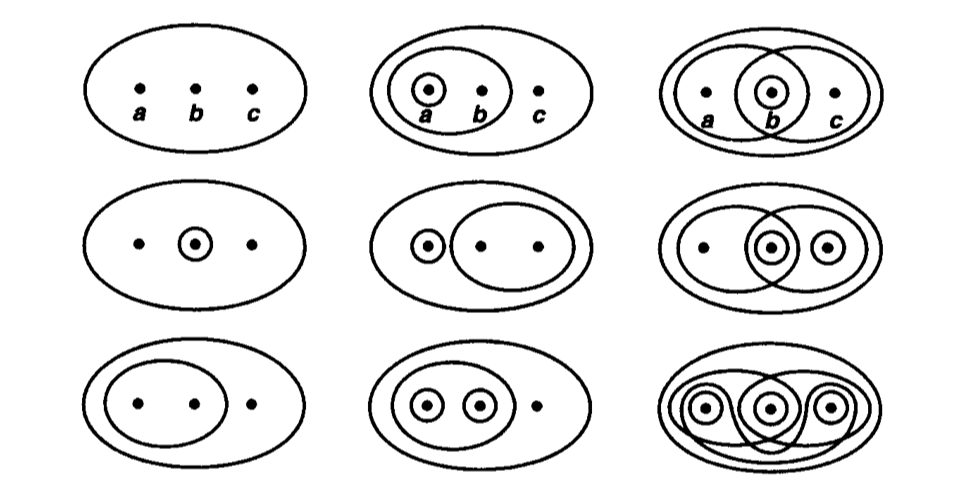
\includegraphics[scale=.75]{top_ex.png}
	\end{center}
\end{figure}
\end{exercise}
\begin{solution}
	We'll label the examples by the coordinates $(i,j)$ where $i,j \in \{1,2,3\}$ correspond to the row/column number. Then, in the matrix below, we'll list which pair is finer, or ``inc'' if the pair is incomparable. 
	\begin{center}
	\begin{tabular}{ |c|c|c|c|c|c|c|c|c|c| } 	
		\hline
		& (1,1) & (1,2) & (1,3) & (2,1) & (2,2) & (2,3) & (3,1) & (3,2) & (3,3) \\	
		\hline
		(1,1) & = & (1,2) & (1,3) & (2,1) & (2,2) & (2,3) & (3,1) & (3,2) & (3,3) \\
		\hline 
		(1,2) & & = & inc & inc & inc & inc & (1,2) & (3,2) & (3,3) \\
		\hline
		(1,3) & & & = & (1,3) & inc & (2,3) & (1,3) & inc & (3,3) \\
		\hline
		(2,1) & & & & = & inc & (2,3) & inc & (3,2) & (3,3)\\
		\hline
		(2,2) & & & & & = & inc & inc & inc & (3,3) \\
		\hline
		(2,3) & & & & & & = & (2,3) & inc & (3,3) \\
		\hline
		(3,1) & & & & & & & = & (3,2) & (3,3) \\
		\hline
		(3,2) & & & & & & & & = & (3,3) \\
		\hline
		(3,3) & & & & & & & & & = \\ 
		\hline
	\end{tabular}
	\end{center}
\end{solution}

\begin{exercise}
	Show $\tT_c$ is a topology: Let $X$ be a set. Let $\tT_c$ be the collection of all subsets of $U$ of $X$ such that $X-U$ either is countable or is all of $X$. 
\end{exercise}
\begin{solution}
	We check the three conditions:
	\begin{enumerate}
		\item $X - \emptyset = X$ is all of $X$, so $\emptyset \in \tT_c$. $X - X = \emptyset$, which is finite, so $X \in \tT_c$.
		\item Let $\{U_\alpha\}$ be an indexed family of nonempty elements of $\tT_c$. Note that for each $\alpha$, $X - U_\alpha$ is countable. Then
		\begin{equation}
			X - \bigcup U_\alpha = \bigcap (X - U_\alpha)
		\end{equation}
		The intersection of countable sets is also countable, so $\{U_\alpha\} \in \tT_c$.
		\item Let $\{U_i\}_{i=1}^n$ be nonempty elements of $\tT_c$. Then
		\begin{equation}
			X - \bigcap_{i=1}^n U_i = \bigcup_{i=1}^n (X - U_i)
		\end{equation}
		The finite union of countable sets is also finite, so that $\{U_i\}_{i=1}^n \in \tT_c$.
	\end{enumerate}
\end{solution}

\begin{exercise}
	Is the collection $\tT_\infty = \{U | X-U \text{ is infinite or empty or all of $X$ } \}$ a topology on $X$?
\end{exercise}
\begin{solution}
	No. Counter example: 
\end{solution}



\end{document}